\subsection{音声合成法}
\subsubsection{全体像}
本実験で用いる学習データセット$\datasetTrain$を
\begin{equation}
    \datasetTrain = \lrc{\lr{\video, \spWaveformGt, \spkEmb, \melGt, \hubertIntGt, \hubertDiscGt}}_{\numLower = 1}^{\numUpper}
\end{equation}
とする.各$\numLower$に対し,$\video \in \videoSet$は口唇動画, $\spWaveformGt \in \spWaveformSet$は原音声の音声波形,$\spkEmb \in \spkEmbSet$は話者ベクトル,$\melGt \in \melSet$はメルスペクトログラム,$\hubertIntGt \in \hubertIntSet$はHuBERT中間特徴量,$\hubertDiscGt \in \hubertDiscGtSet$はHuBERT離散特徴量とする.$T$に添字をつけて各サンプル$n$ごとの各特徴量の系列長,$D$に添字をつけて各特徴量の次元,$W, H$で動画の幅と高さ,$C$でクラス数を表した.以下,新たに定義される変数も同様の表記でデータの形状を表した.

ここで,話者ベクトル$\spkEmb$は,話者識別モデル\cite{wan2018generalized}を利用して得られた音声の話者性を反映するベクトル(d-vector)である.話者識別モデルは,LSTMと全結合層から構成され,softmax関数を用いたGeneralized End-to-End Lossを用いて学習される.これは,各話者ごとに複数の発話から得られた話者ベクトルの平均を重心とし,各話者ベクトルについて同一話者の重心とのコサイン類似度を最大化し,異なる話者の重心とのコサイン類似度を最小化するように設計された損失関数である.よって,学習されたモデルによって得られる話者ベクトルは,話者間での識別性を有したベクトルとなる.本実験ではこれをモデルへの入力とすることで,動画から音声を予測する際に話者性を正しく反映させることを狙った.

また,HuBERT中間特徴量とHuBERT離散特徴量は,HuBERTを利用して得られる特徴量である.HuBERTは,1次元畳み込み層を中心とした畳み込みエンコーダとTransformerから構成され,Masked Predictionによって学習される.これは,音声波形を畳み込みエンコーダに通すことで特徴量に変換し,その一部区間をマスクしてからTransformerに入力して,マスクされた区間の教師ラベルを予測させる学習方法である.損失関数には,マスクされた区間に限定したCross Entropy Lossが用いられる.ここで,教師ラベルは学習の過程で更新されるため,学習は2段階に分かれる.1段階目は,MFCCをk-means法によってクラスタリングした結果を教師ラベルとする.2段階目は,1段階目の学習済みモデルのTransformerにおける中間特徴量をk-means法によってクラスタリングした結果を教師ラベルとする.比較的単純なMFCCベースのラベルから,DNNによって得られるより複雑なラベルへと予測対象を更新して学習難易度を高めることで,モデルの表現力を向上させる仕組みとなっている.HuBERTは,マスクされた入力から教師ラベルを予測する学習を行うため,特に音声の文脈的構造を学習可能だと考えられる.ここで,HuBERTにおける畳み込みエンコーダまでを$\hubertConv$,HuBERTにおけるTransformerを$\hubertTransformer$,k-means法を$\kmeans$,インデックス系列をOne-hotベクトルに変換する関数を$\onehot$とすると,HuBERT中間特徴量$\hubertIntGt$およびHuBERT離散特徴量$\hubertDiscGt$は,
\begin{gather}
    \hubertIntGt = \hubertConv\lr{\spWaveformGt; \weightHuBERTConv} \\
    \hubertDiscGt = \onehot\lr{\kmeans\lr{\hubertTransformer\lr{\hubertIntGt; \weightHuBERTTrans}}}
\end{gather}
で与えられる.ここで,$\weightHuBERTConv, \weightHuBERTTrans$はHuBERTの事前学習済み重みを表す.Masked Predictionにおいてマスク対象となっていたのは,ここで定めたHuBERT中間特徴量にあたる.

提案手法を図\ref{sec4:fig:overview}に示す.赤の平行四辺形が入出力,青の長方形が処理を表す.提案手法は,ネットワークA,ネットワークB,ボコーダの3つからなる.まず,ネットワークAを$\myNetworkA$とすると,$\myNetworkA$の行う処理は,
\begin{equation}
    \label{sec4:eq:networkA_overview}
    \hubertIntPred, \melPredA, \hubertDiscPredA = \myNetworkA\lr{\video, \spkEmb; \weightA}
\end{equation}
と表される.ここで,$\hubertIntPred \in \hubertIntSet$は予測HuBERT中間特徴量,$\melPredA \in \melSet$はネットワークAの予測メルスペクトログラム,$\hubertDiscPredA \in \hubertDiscPredSet$はネットワークAのHuBERT離散特徴量に対するロジットを表す.次に,ネットワークBを$\myNetworkB$とすると,$\myNetworkB$の行う処理は,
\begin{equation}
    \melPredB, \hubertDiscPredB = \myNetworkB\lr{\hubertIntPred, \spkEmb; \weightB}
\end{equation}
と表される.ここで,$\melPredB \in \melSet$はネットワークBの予測メルスペクトログラム,$\hubertDiscPredB \in \hubertDiscPredSet$はネットワークBのHuBERT離散特徴量に対するロジットを表す.最後に,音声波形を生成するボコーダを$\vocoder$とすると,$\vocoder$の行う処理は,
\begin{equation}
    \spWaveformPred = \vocoder\lr{\melPredB, \hubertDiscPredB; \weightVoc}
\end{equation}
と表される.まとめると,提案手法は口唇動画と話者ベクトルを入力とし,ネットワークAとネットワークBによって中間表現を獲得後,これをボコーダに入力することで音声波形を生成するものである.

\begin{figure}[bt]
    \centering
    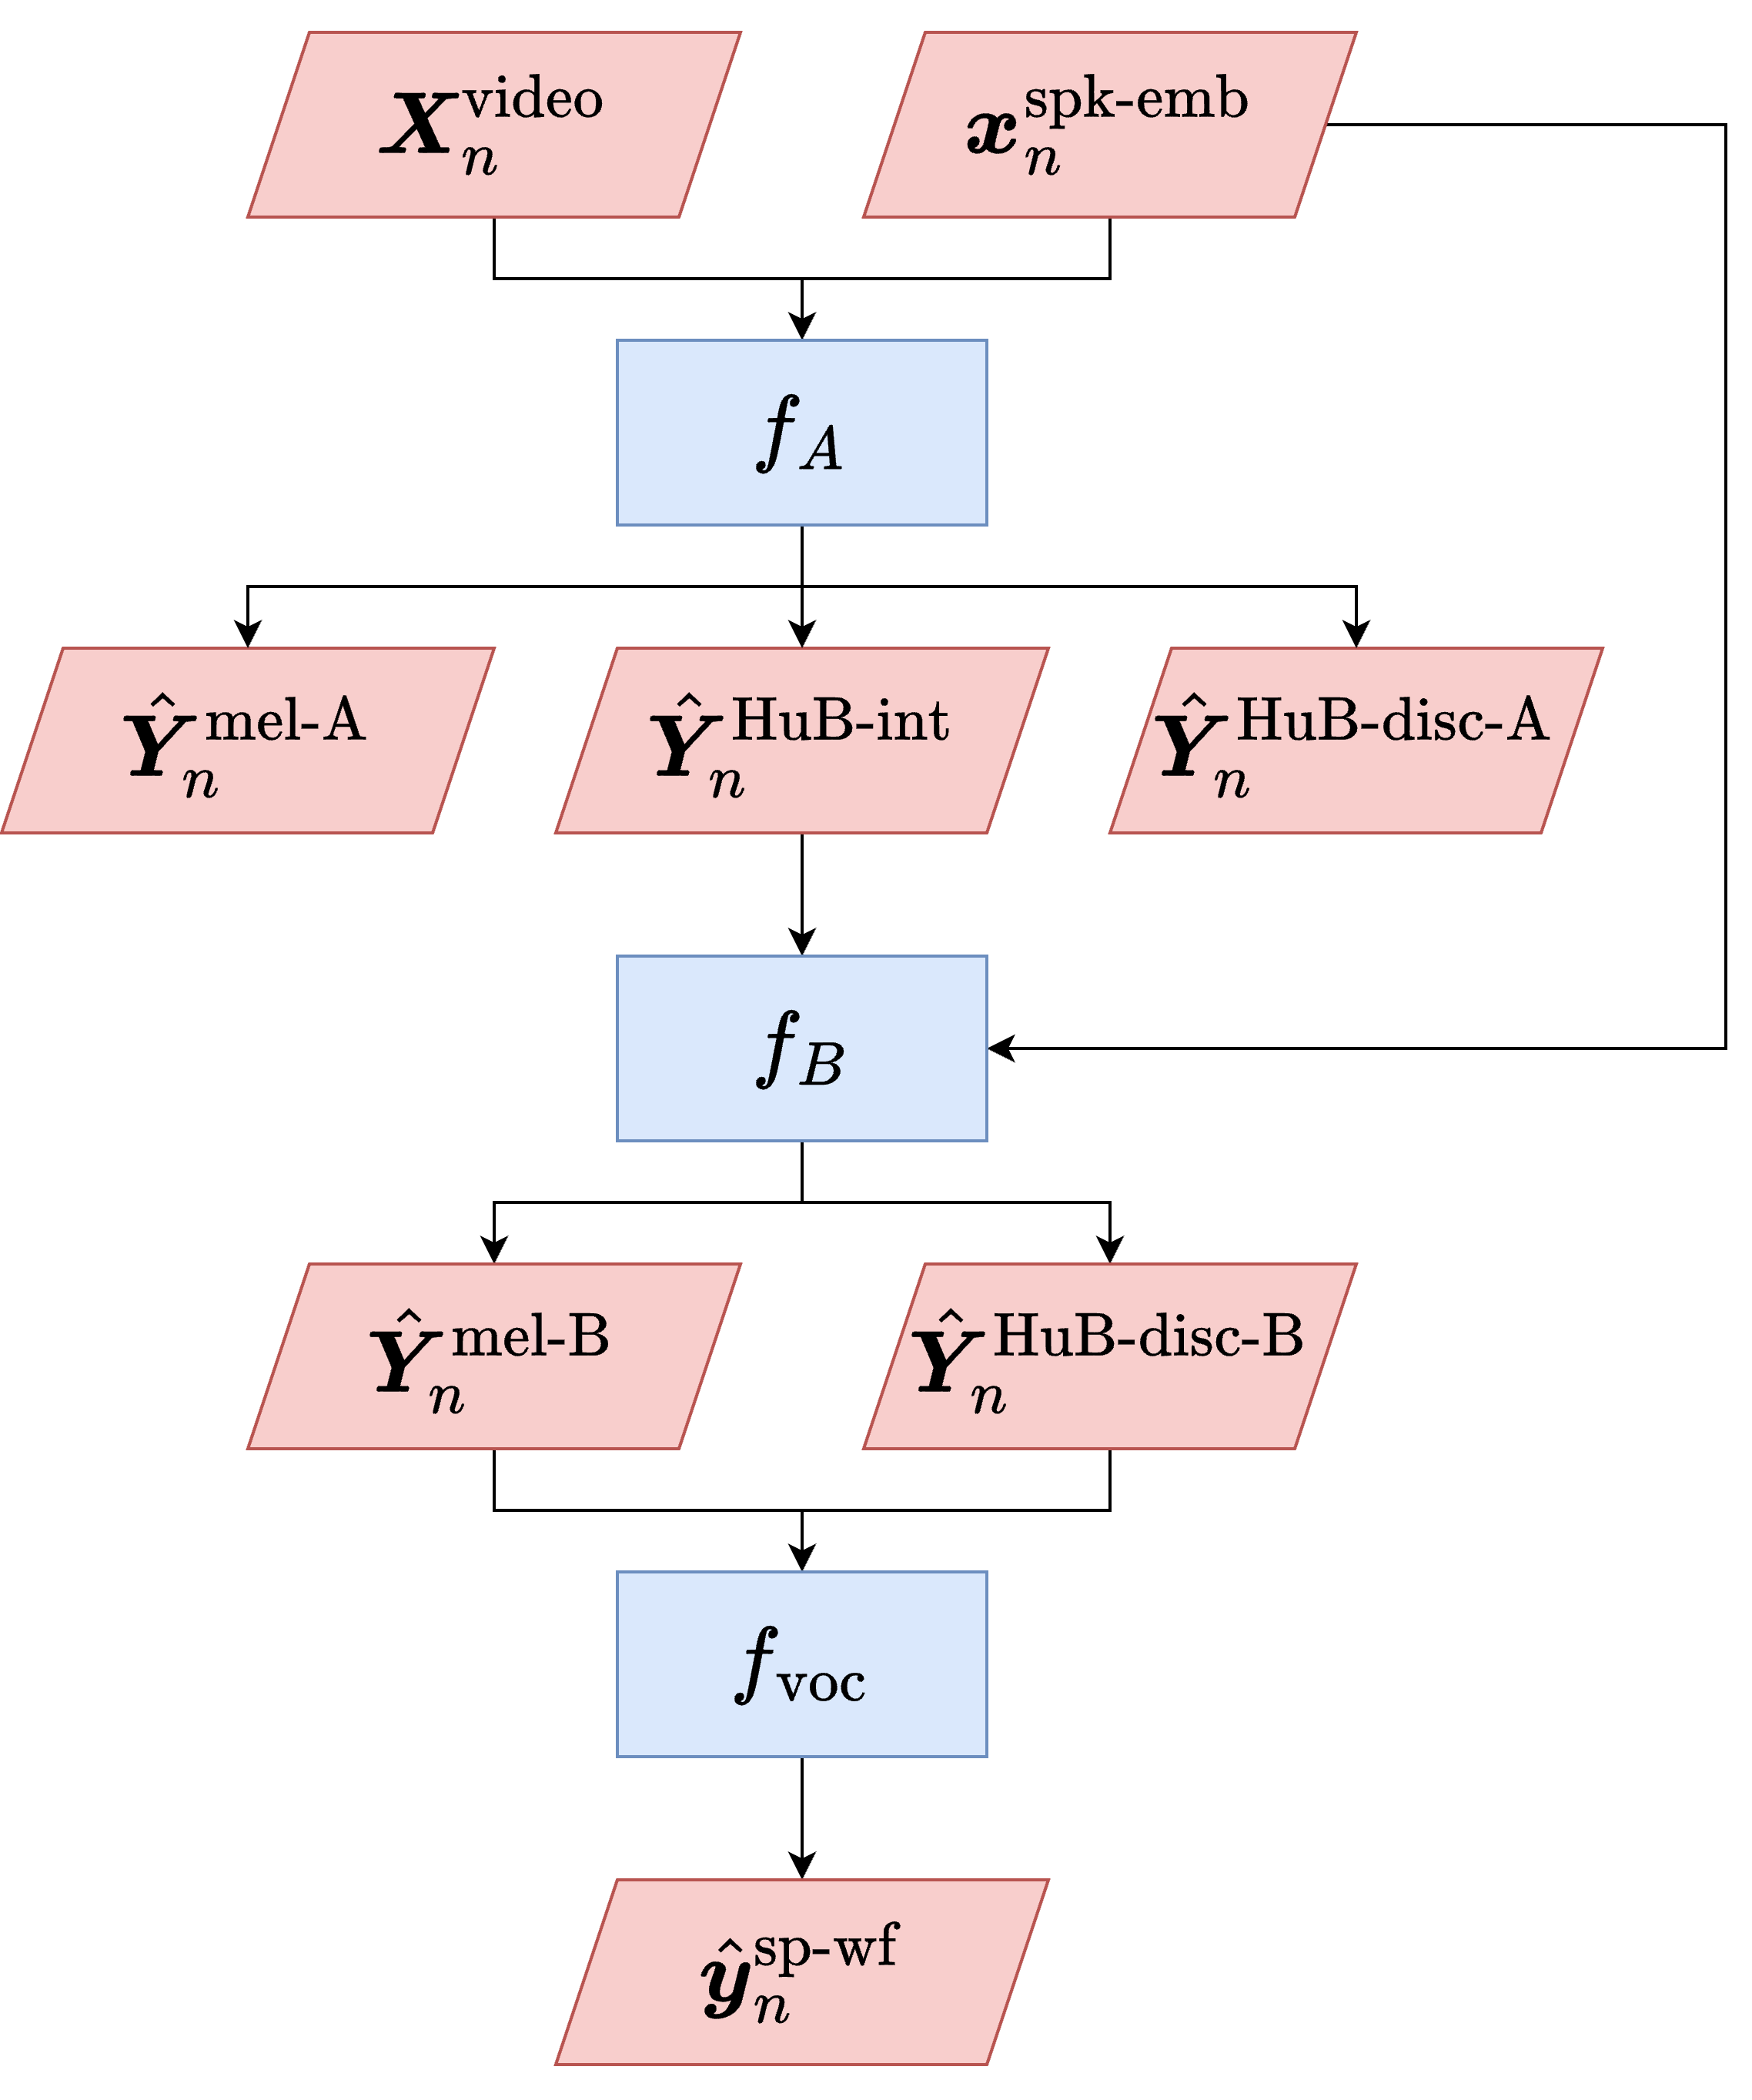
\includegraphics[height=100mm]{./figure/sec4/model_2/overview.drawio.png}
    \caption{提案手法の全体像(赤い平行四辺形:入出力,青い長方形:処理)}
    \label{sec4:fig:overview}
\end{figure}

\subsubsection{ネットワークA}
ネットワークAを図\ref{sec4:fig:networkA}に示す.赤の平行四辺形が入出力,青の長方形が処理を表す.ネットワークAでは,まず,口唇動画$\video$をAVHuBERTに通すことで,特徴量$\featureA \in \featureASet$に変換する.これは,
\begin{equation}
    \featureA = \AVHuBERT\lr{\video; \weightAAVHuBERT}
\end{equation}
と表される.$\weightAAVHuBERT$は,AVHuBERTの事前学習済み重みで初期化した.AVHuBERTは,動画入力に対する3次元畳み込み層と2次元畳み込み層を中心としたResNet,メルスペクトログラム入力に対する全結合層,これらの出力を次元方向に結合した特徴量を入力とするTransformerから構成され,HuBERTと同様にMasked Predictionによって学習される.AVHuBERTでは,動画およびメルスペクトログラムに対してマスクが適用され,マスクされた区間の教師ラベルを予測させる.損失関数には,マスクされた区間に限定したCross Entropy Lossが用いられる.また,ResNetから出力される動画特徴量と,全結合層から出力される音声特徴量を次元方向に結合する前には,Modality Dropoutが行われる.これは,各フレームにおいて両方のモダリティを入力とするか,どちらか一方のモダリティのみを入力とする(他方を0に置き換える)かを確率的に選択するものである.これにより,どちらか一方のモダリティのみに依存しないようにモデルを学習させることが可能となるため,特定のタスクにFineTuningする際には,Masked Predictionを行う場合のように動画と音声の両方を入力とせず,どちらか一方のモダリティのみを入力としても破綻しないよう設計されている.また,AVHuBERTでも,HuBERTと同様に教師ラベルの更新を段階的に行う.1段階目はMFCCをk-means法によってクラスタリングした結果を教師ラベルとし,2から5段階目は前回の学習済みモデルのTransformerにおける中間特徴量をk-means法によってクラスタリングした結果を教師ラベルとする.比較的単純なMFCCベースのラベルから,DNNによって得られるより複雑なラベルへと予測対象を更新して学習難易度を高めることで,モデルの表現力を向上させる仕組みとなっている.AVHuBERTは,HuBERTと同様に動画および音声の文脈的構造を学習可能だと考えられるが,さらに2つのモダリティが組み合わさることで,これらの対応関係なども合わせたより複雑な関係性が学習可能だと考えられる.動画音声合成では,先行研究においてAVHuBERTを転移学習することの有効性がすでに示されているため,本実験においても採用した.

次に,$\featureA$の各時刻$t$におけるベクトルに対し,話者ベクトル$\spkEmb$を次元方向に結合してから,全結合層によって次元を再度圧縮し,元の次元に戻す.これは,
\begin{equation}
    \featureA = \myNetworkSpkMerge\lr{\concat{\featureA, \spkEmb \bm{1}^{\top}}; \weightAFcSpk}
\end{equation}
と表される.ここで,$\bm{1} \in \{1\}^{\timeUpper^{\text{video}}_{\numLower}}$は全成分が1のベクトルである.次に,話者ベクトルが統合された特徴量に対する後処理として,$\myNetworkPost$を適用する.これは,
\begin{equation}
    \featureA = \myNetworkPost\lr{\featureA; \weightAPost}
\end{equation}
と表される.ここで,後処理層$\myNetworkPost$の構造を図\ref{sec4:fig:post_three_step}に示す.赤の平行四辺形が入出力,青の長方形が処理を表す.内部特徴量は全て$\bm{H}_{\numLower}$で表した.$\myNetworkPost$は,1次元畳み込み層を中心としたConvBlockおよび,これに残差結合を組み合わせたResBlockから構成される.$\myNetworkPost$は,話者ベクトル$\spkEmb$が次元方向に結合された特徴量$\featureA$に対する話者性を考慮した変換を行うために導入した.なぜなら,$\AVHuBERT$はMasked Predictionによって事前学習されたモデルだから,動画の文脈的な構造を考慮するのに適していると考えられる一方で,音声合成に必要となる話者性は発話に依存しない,動画の文脈的な構造とは別の性質を持った情報だと考えたからである.

最後に,$\featureA$を全結合層を通して変換することで,予測対象であるHuBERT中間特徴量,メルスペクトログラム,HuBERT離散特徴量に対するロジットを得る.これは,
\begin{gather}
    \hubertIntPred = \myNetworkFcHubInt\lr{\featureA; \weightAFcHubInt} \\
    \melPredA = \myNetworkFcMel\lr{\featureA; \weightAFcMel} \\
    \hubertDiscPredA = \myNetworkFcHubDisc\lr{\featureA; \weightAFcHuBDisc}
\end{gather}
と表される.$\weightAFcSpk, \weightAPost, \weightAFcHubInt, \weightAFcMel, \weightAFcHuBDisc$は,すべてランダムに初期化した.

ネットワークAの役割は,続くネットワークBの入力であるHuBERT中間特徴量を予測することである.これに対し,メルスペクトログラムとHuBERT離散特徴量の予測を同時に行った理由は,先行研究においてマルチタスク学習の有効性が確認されており,HuBERT中間特徴量の予測においても有効ではないかと考えたからである.

\begin{figure}[tb]
    \centering
    \begin{subfigure}[b]{0.48\textwidth}
        \centering
        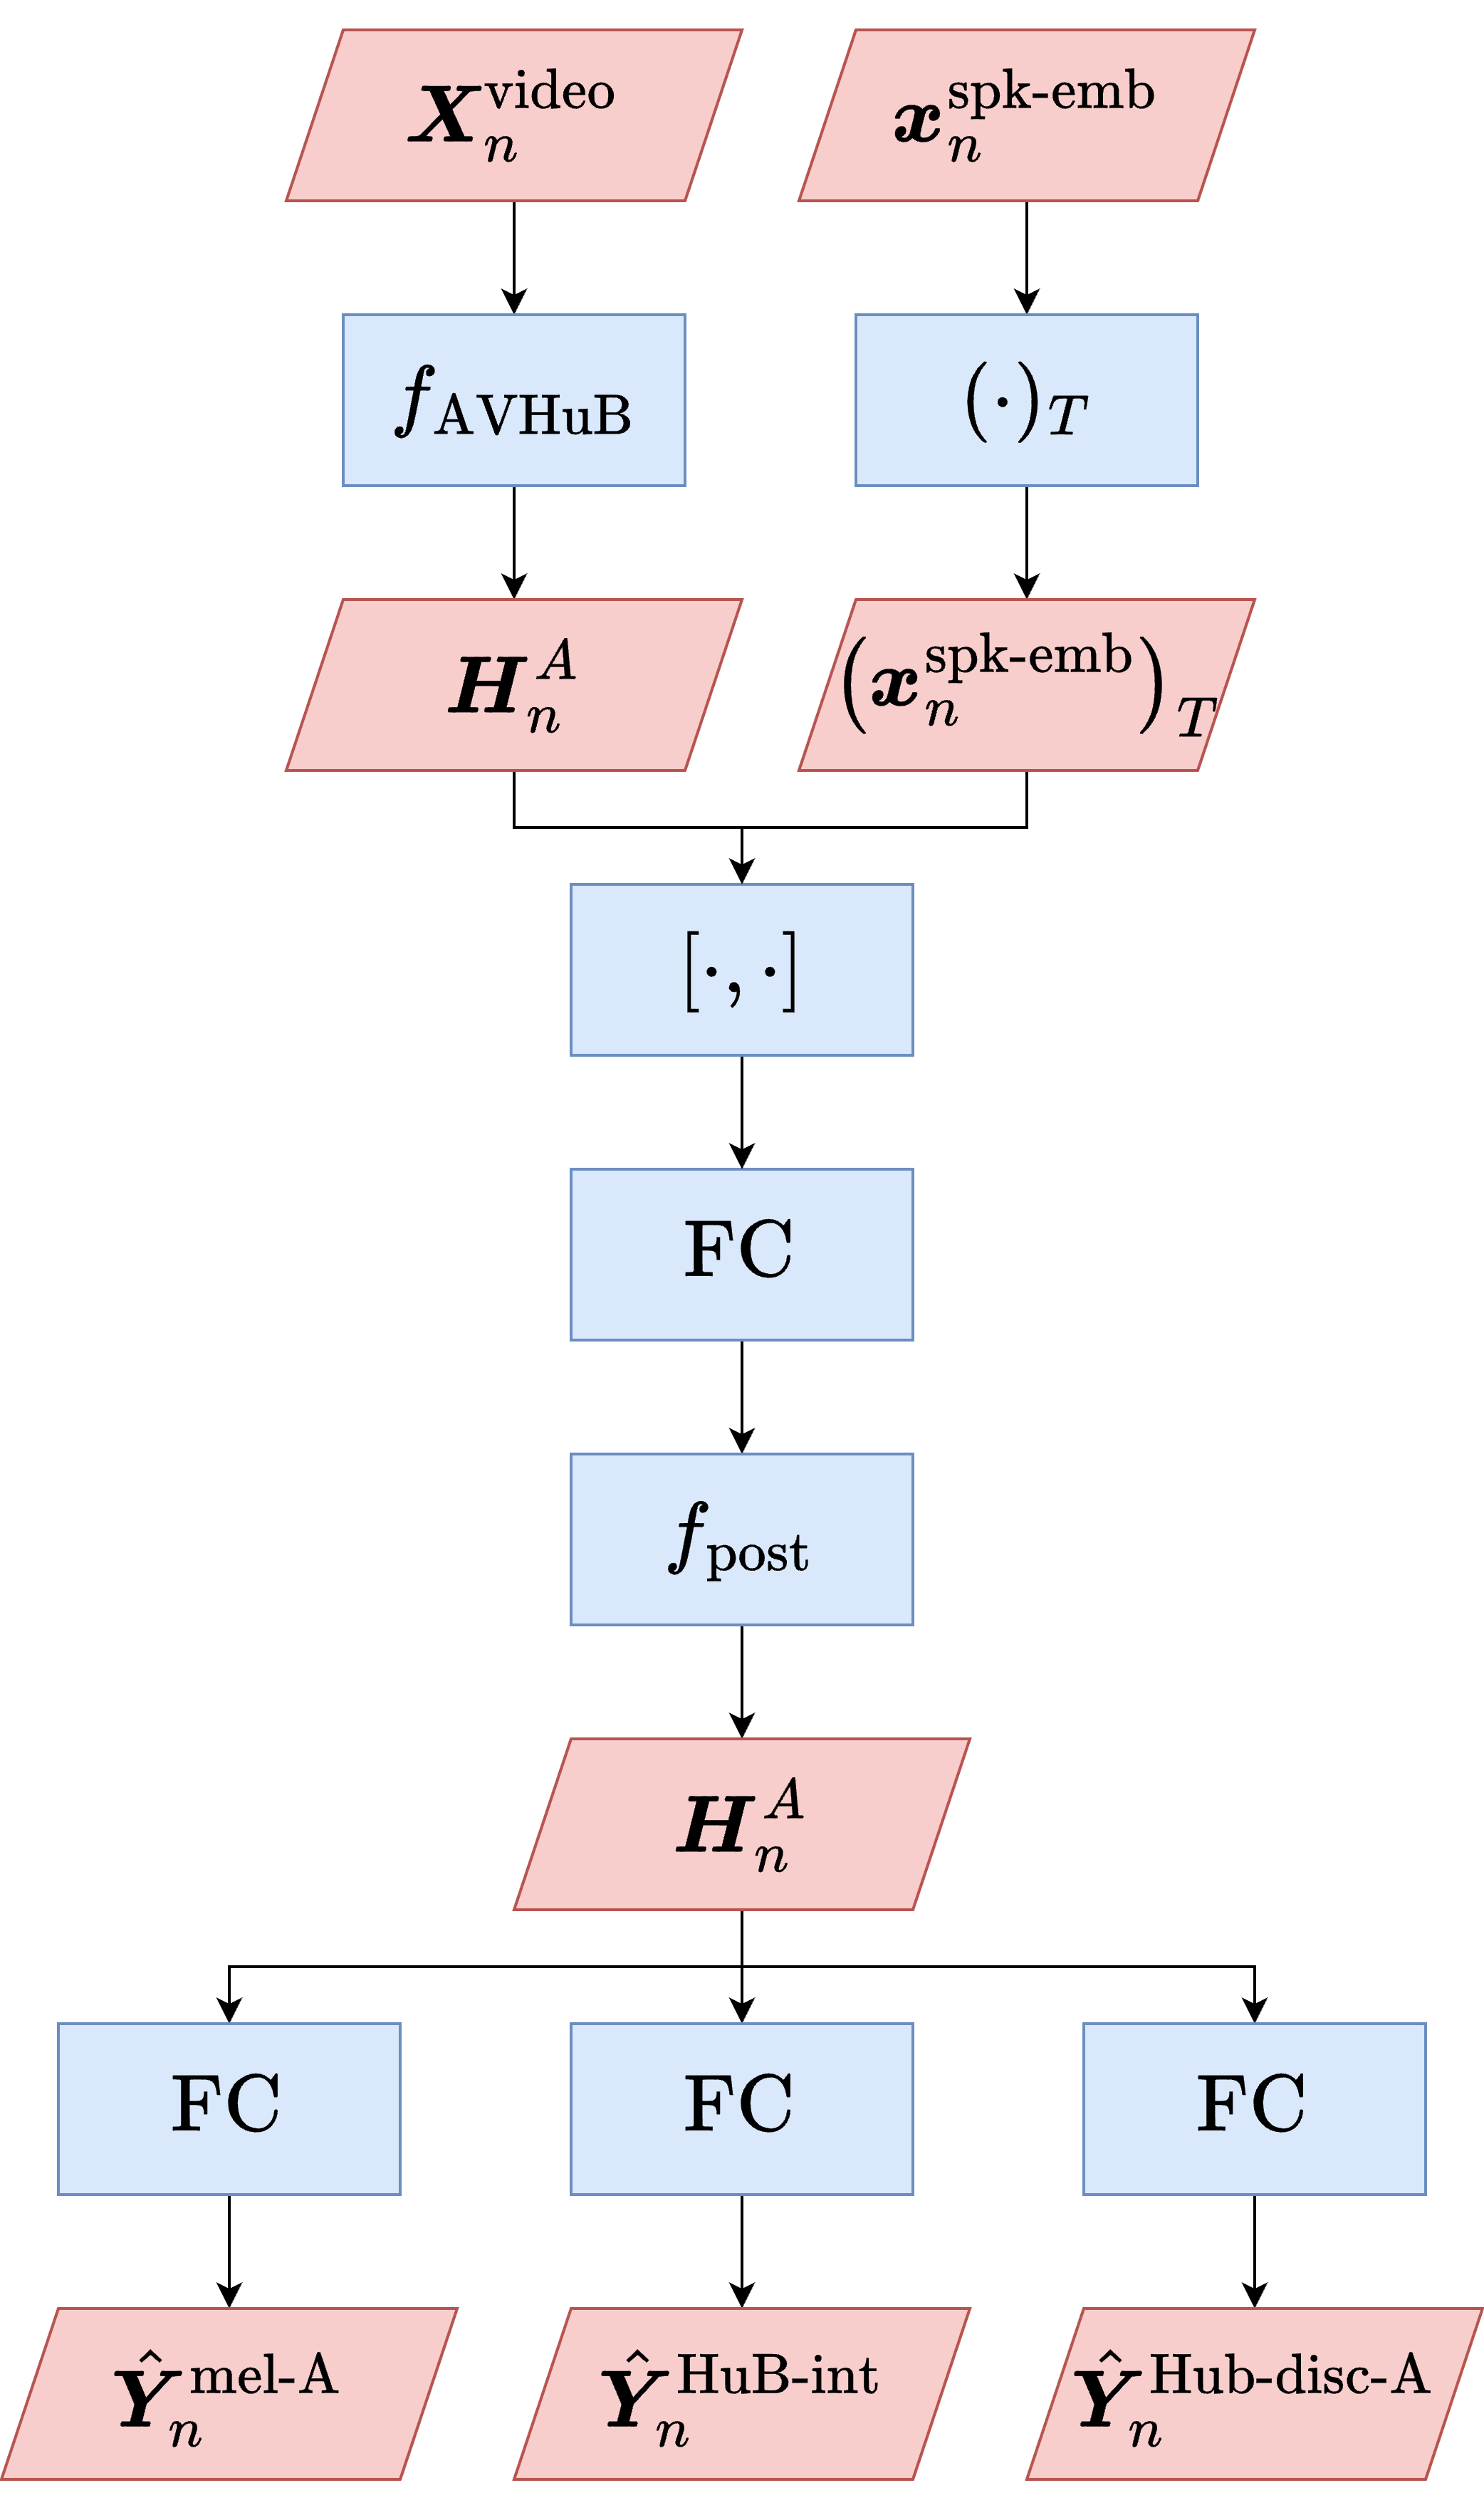
\includegraphics[height=120mm]{./figure/sec4/model_2/networkA.drawio.png}
        \caption{ネットワークA}
        \label{sec4:fig:networkA}
    \end{subfigure}
    \hfill
    \begin{subfigure}[b]{0.48\textwidth}
        \centering
        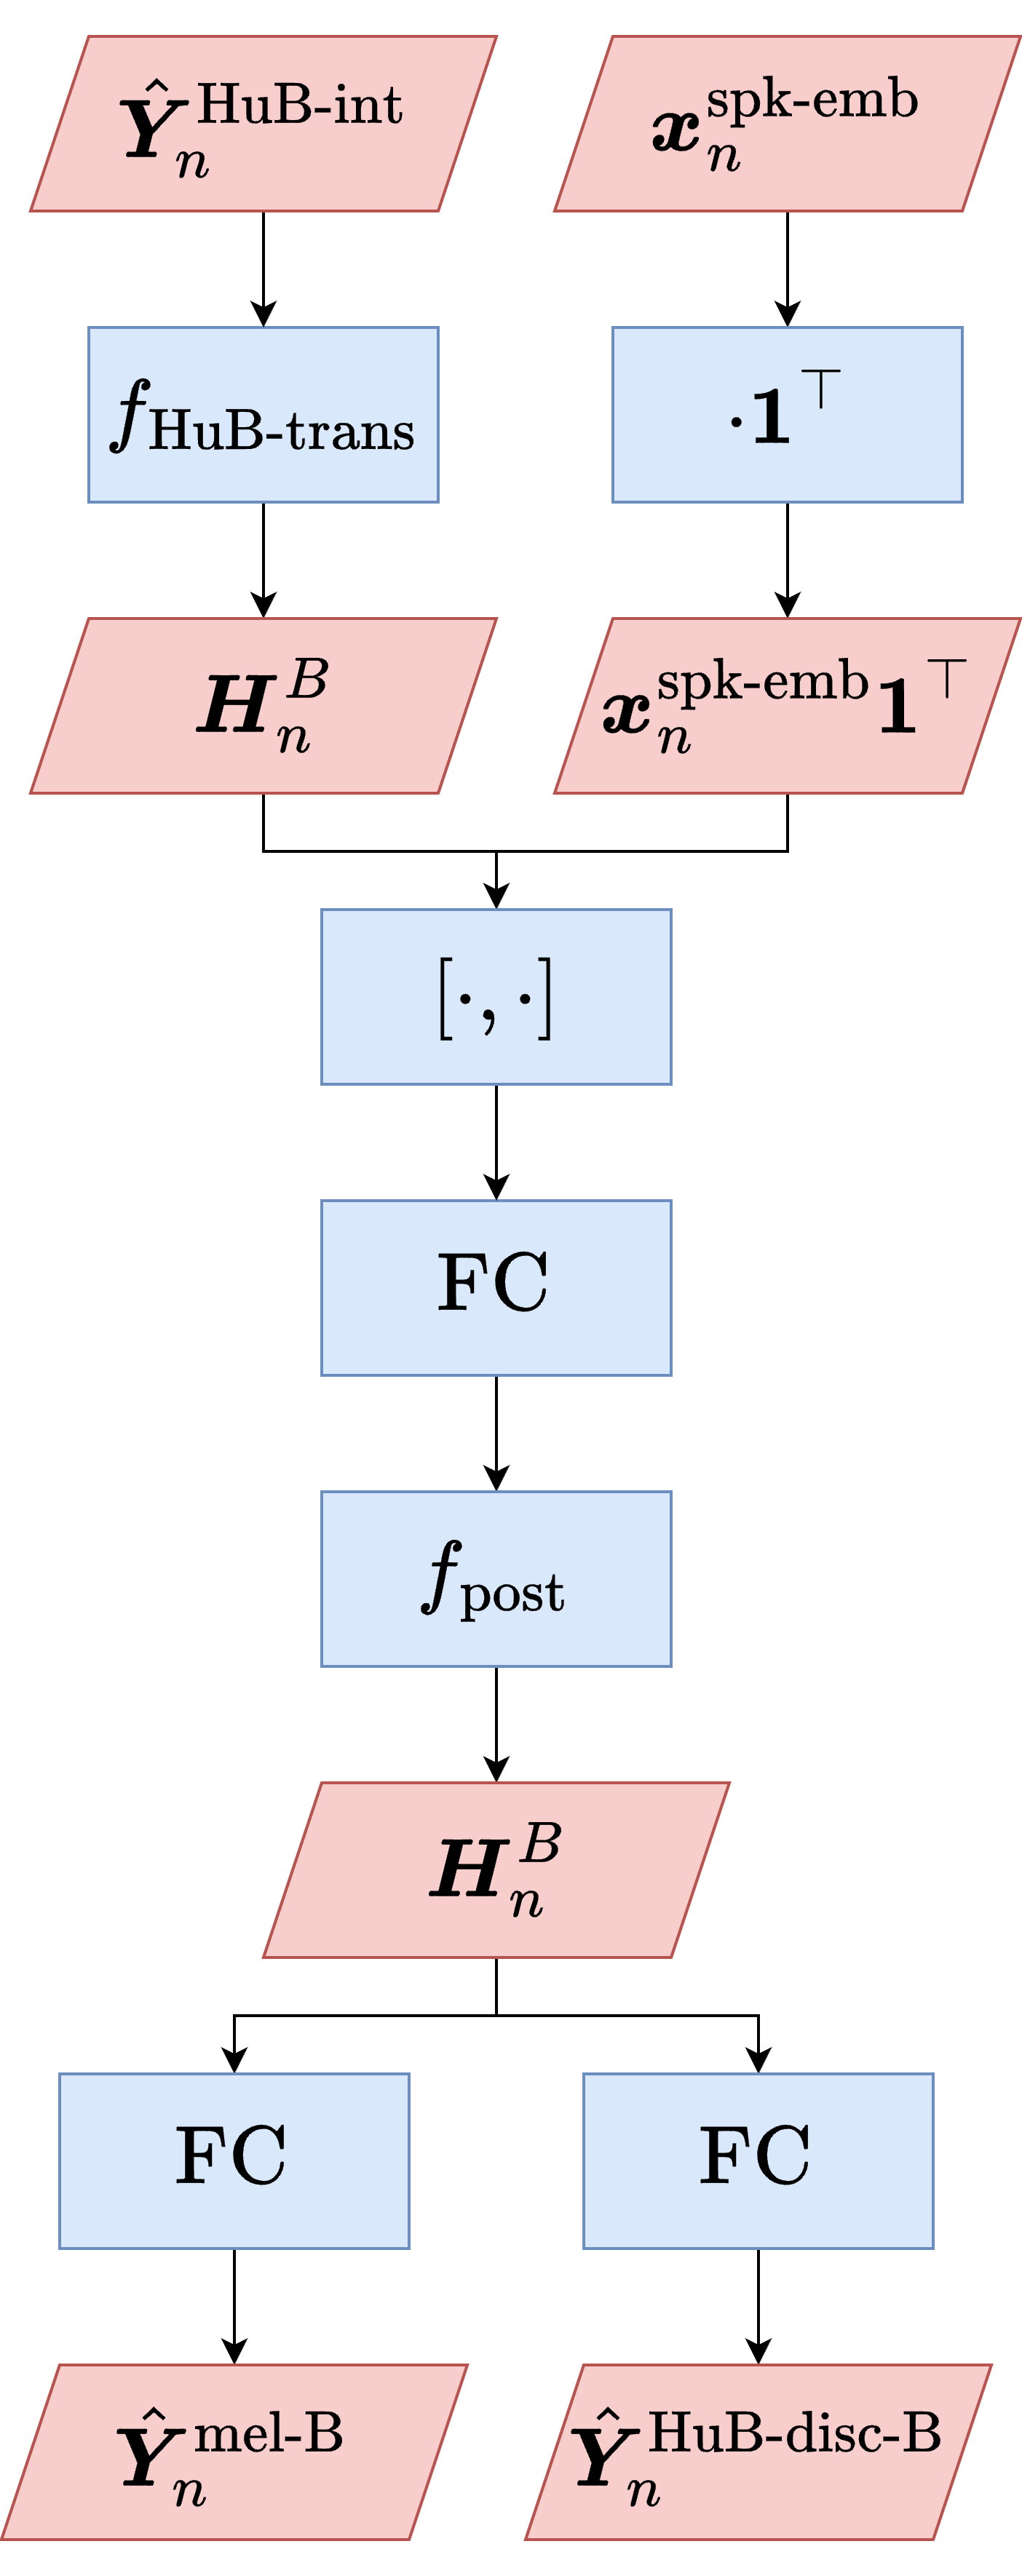
\includegraphics[height=120mm]{./figure/sec4/model_2/networkB.drawio.png}
        \caption{ネットワークB}
        \label{sec4:fig:networkB}
    \end{subfigure}
    \hfill
    \caption{ネットワークAとネットワークBの構造(赤い平行四辺形:入出力,青い長方形:処理)}
    \label{sec4:fig:networkAB}
\end{figure}

\begin{figure}[tb]
    \centering
    \begin{subfigure}[b]{0.32\textwidth}
        \centering
        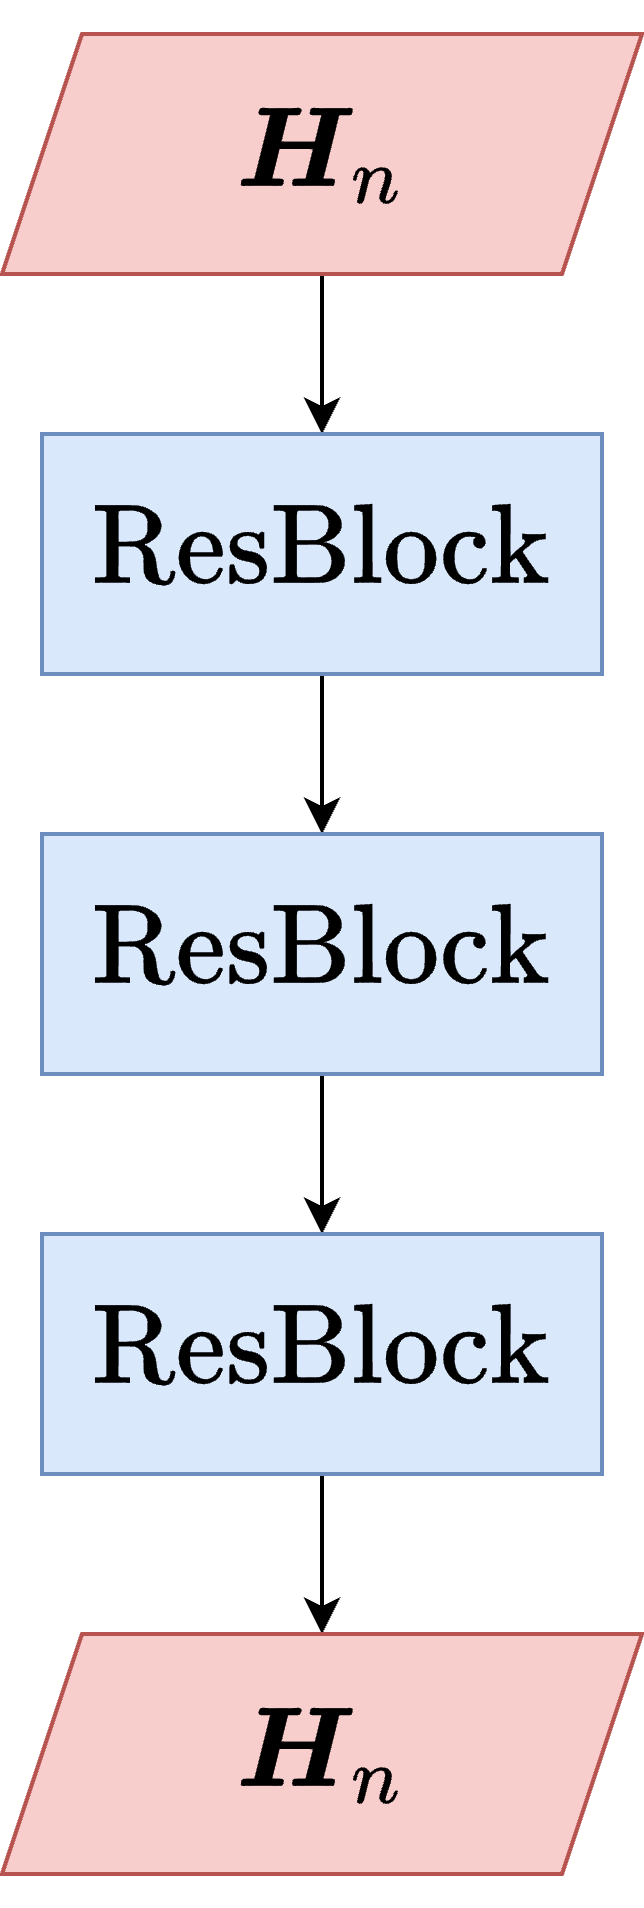
\includegraphics[height=70mm]{./figure/sec4/model_2/post.drawio.png}
        \caption{全体}
        \label{sec4:fig:post}
    \end{subfigure}
    \hfill
    \begin{subfigure}[b]{0.32\textwidth}
        \centering
        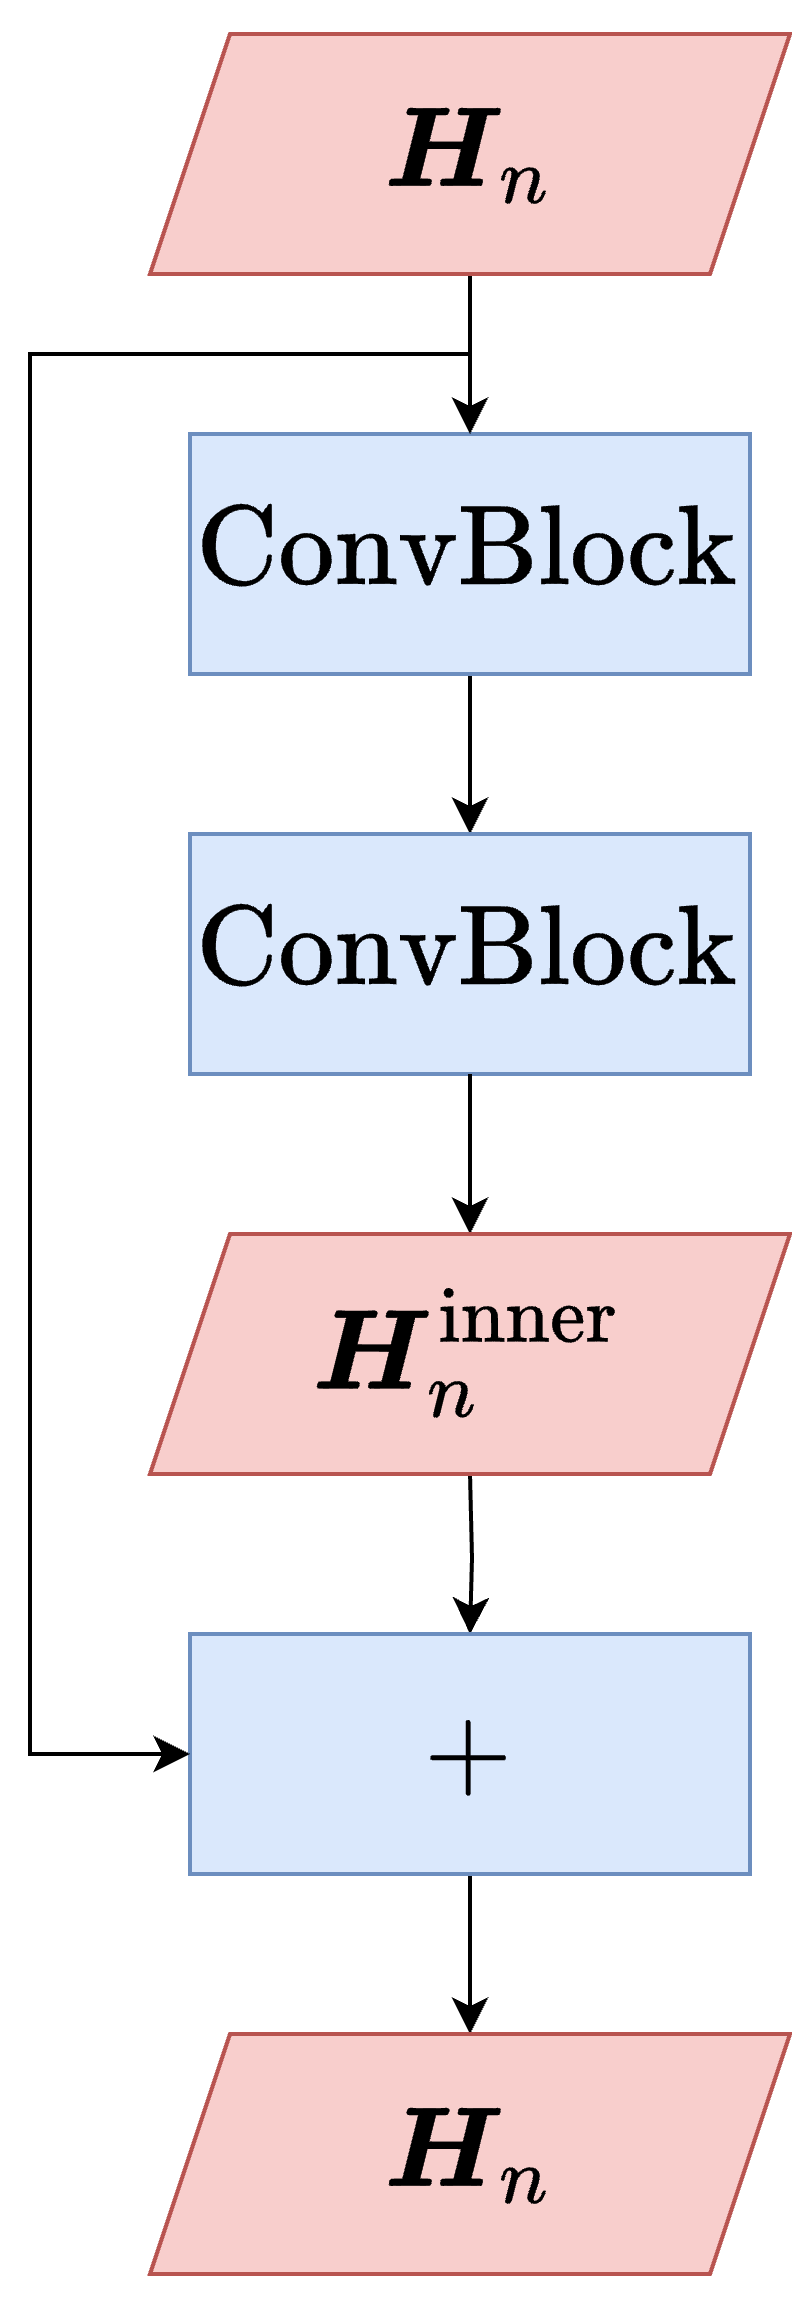
\includegraphics[height=70mm]{./figure/sec4/model_2/post_resblock.drawio.png}
        \caption{ResBlock}
        \label{sec4:fig:post_resblock}
    \end{subfigure}
    \hfill
    \begin{subfigure}[b]{0.32\textwidth}
        \centering
        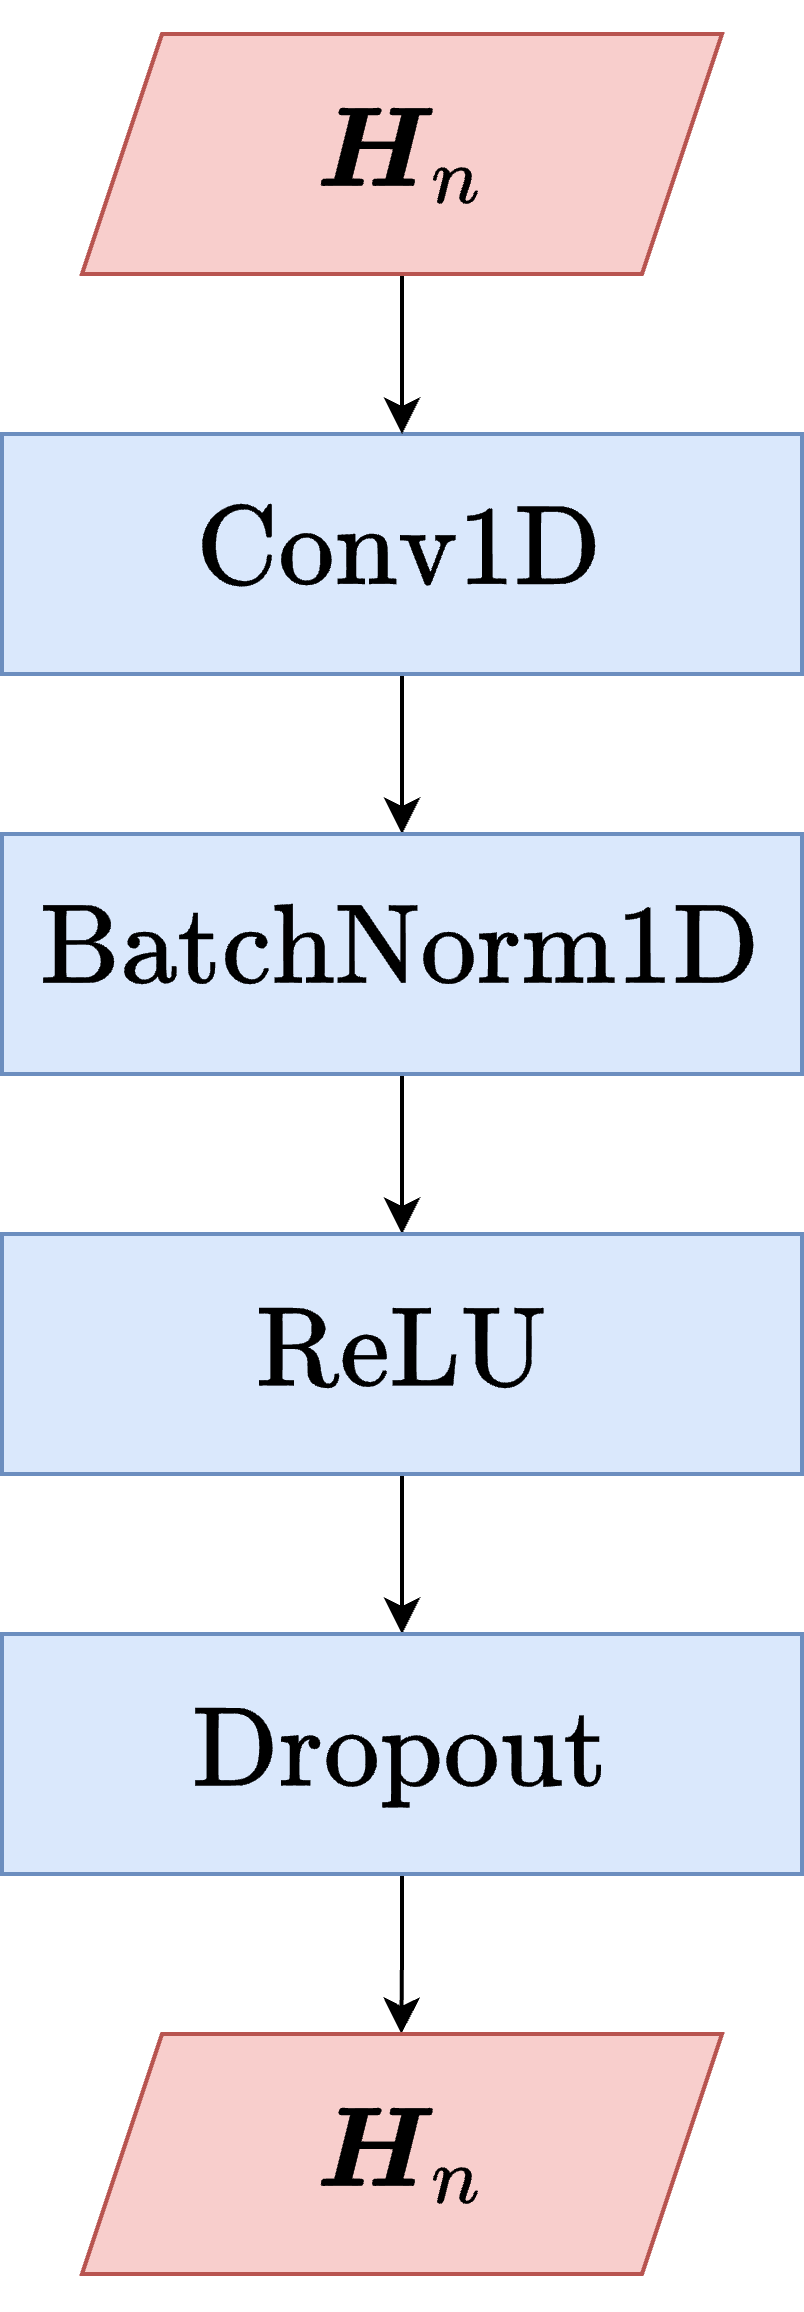
\includegraphics[height=70mm]{./figure/sec4/model_2/post_convblock.drawio.png}
        \caption{ConvBlock}
        \label{sec4:fig:post_convblock}
    \end{subfigure}
    \caption{後処理層$\myNetworkPost$の構造(赤い平行四辺形:入出力,青い長方形:処理)}
    \label{sec4:fig:post_three_step}
\end{figure}

\subsubsection{ネットワークB}
ネットワークBを図\ref{sec4:fig:networkB}に示す.赤の平行四辺形が入出力,青の長方形が処理を表す.ネットワークBでは,まず,ネットワークAで得られた予測HuBERT中間特徴量$\hubertIntPred$を$\hubertTransformer$に通すことで,特徴量$\featureB \in \featureBSet$に変換する.これは,
\begin{equation}
    \featureB = \hubertTransformer\lr{\hubertIntPred; \weightBHuBERTTrans}
\end{equation}
と表される.$\weightBHuBERTTrans$は,HuBERTの事前学習済み重みで初期化する場合と,ランダム初期化する場合の2つを検討した.以下,ネットワークAと処理は同様であるため,数式のみ記載する.
\begin{gather}
    \featureB = \myNetworkSpkMerge\lr{\concat{\featureB, \spkEmb \bm{1}^{\top}}; \weightBFcSpk} \\
    \featureB = \myNetworkPost\lr{\featureB; \weightBPost} \\
    \melPredB = \myNetworkFcMel\lr{\featureB; \weightBFcMel} \\
    \hubertDiscPredB = \myNetworkFcHubDisc\lr{\featureB; \weightBFcHuBDisc}
\end{gather}
$\weightBFcSpk, \weightBPost, \weightBFcMel, \weightBFcHuBDisc$は,すべてランダムに初期化した.

ネットワークBの役割は,メルスペクトログラムとHuBERT離散特徴量の予測である.このネットワークの設計には,HuBERT Transformerが持つ自己教師あり学習の特性を活用する意図がある.HuBERTのMasked Predictionでは,畳み込みエンコーダからの出力にマスクを適用し,Transformerを通じてマスクされたフレームの教師ラベルを予測する.よって,Transformerは不完全な入力をもとに教師ラベルを予測する必要があるため,全体の文脈を考慮して情報を補完する力を持つよう最適化されると考えられる.さらに,HuBERTは音声データのみで学習可能であり,動画音声データの制約を受けず,より大規模なデータセットによる事前学習が可能である.以上の特性に基づき,ネットワークAの不完全な予測結果を,大量の音声データを元に学習された文脈を考慮する力によって補完することで,最終予測値であるメルスペクトログラムとHuBERT離散特徴量に対する予測精度改善を狙った.

\subsubsection{ボコーダ}
ボコーダを図\ref{sec4:fig:vocoder}に示す.赤の平行四辺形が入出力,青の長方形が処理を表す.本実験で用いるボコーダは,今回ベースラインとする先行研究\cite{choi2023intelligible}で提案されたMulti-input Vocoderを参考にしたものである.まず,ネットワークBで得られた予測メルスペクトログラム$\melPredB$とHuBERT離散特徴量に対するロジット$\hubertDiscPredB$を前処理層に通し,扱いやすい形状に変換する.これは,
\begin{gather}
    \featureVocMel = \vocoderPreMel\lr{\melPredB; \weightVocPreMel} \\
    \featureVocHuBERT = \vocoderPreHub\lr{\hubertDiscPredB; \weightVocPreHuB}
\end{gather}
と表される.$\featureVocMel \in \featureVocMelSet$は,$\melPredB$の時間方向に隣接したベクトルを次元方向に結合することで$\hubertDiscPredB$と系列長を揃え,その後全結合層を適用した特徴量である.一方,$\featureVocHuBERT \in \featureVocHuBERTSet$は,$\hubertDiscPredB$に対して$\argmax$関数を適用した後,各時刻$t$において選択されたインデックスをベクトルに変換した特徴量である.次に,$\featureVocMel, \featureVocHuBERT$を入力として,音声波形を生成する.これは,
\begin{equation}
    \spWaveformPred = \vocoderMain\lr{\concat{\featureVocMel, \featureVocHuBERT}; \weightVocMain}
\end{equation}
と表される.$\vocoderMain$は,図\ref{sec4:fig:vocoder_main}に示すように,1次元畳み込み層とUpsamplingBlockから構成され,これはHiFi-GAN\cite{kong2020hifi}のGeneratorと同様である.各UpsamplingBlockでは,初めに1次元転置畳み込み層を通すことで時間方向のアップサンプリングを行い,その後複数の1次元畳み込み層から特徴抽出を行った結果を平均して出力する.図\ref{sec4:fig:vocoder_main_block}において,内部特徴量は$\bm{H}_{\numLower}$で表した.また,$\numUpper_{\text{Conv1D}}$は,UpsamplingBlockに並列に設けられている1次元畳み込み層の数を表す.

\begin{figure}[tb]
    \centering
    \begin{subfigure}[b]{0.32\textwidth}
        \centering
        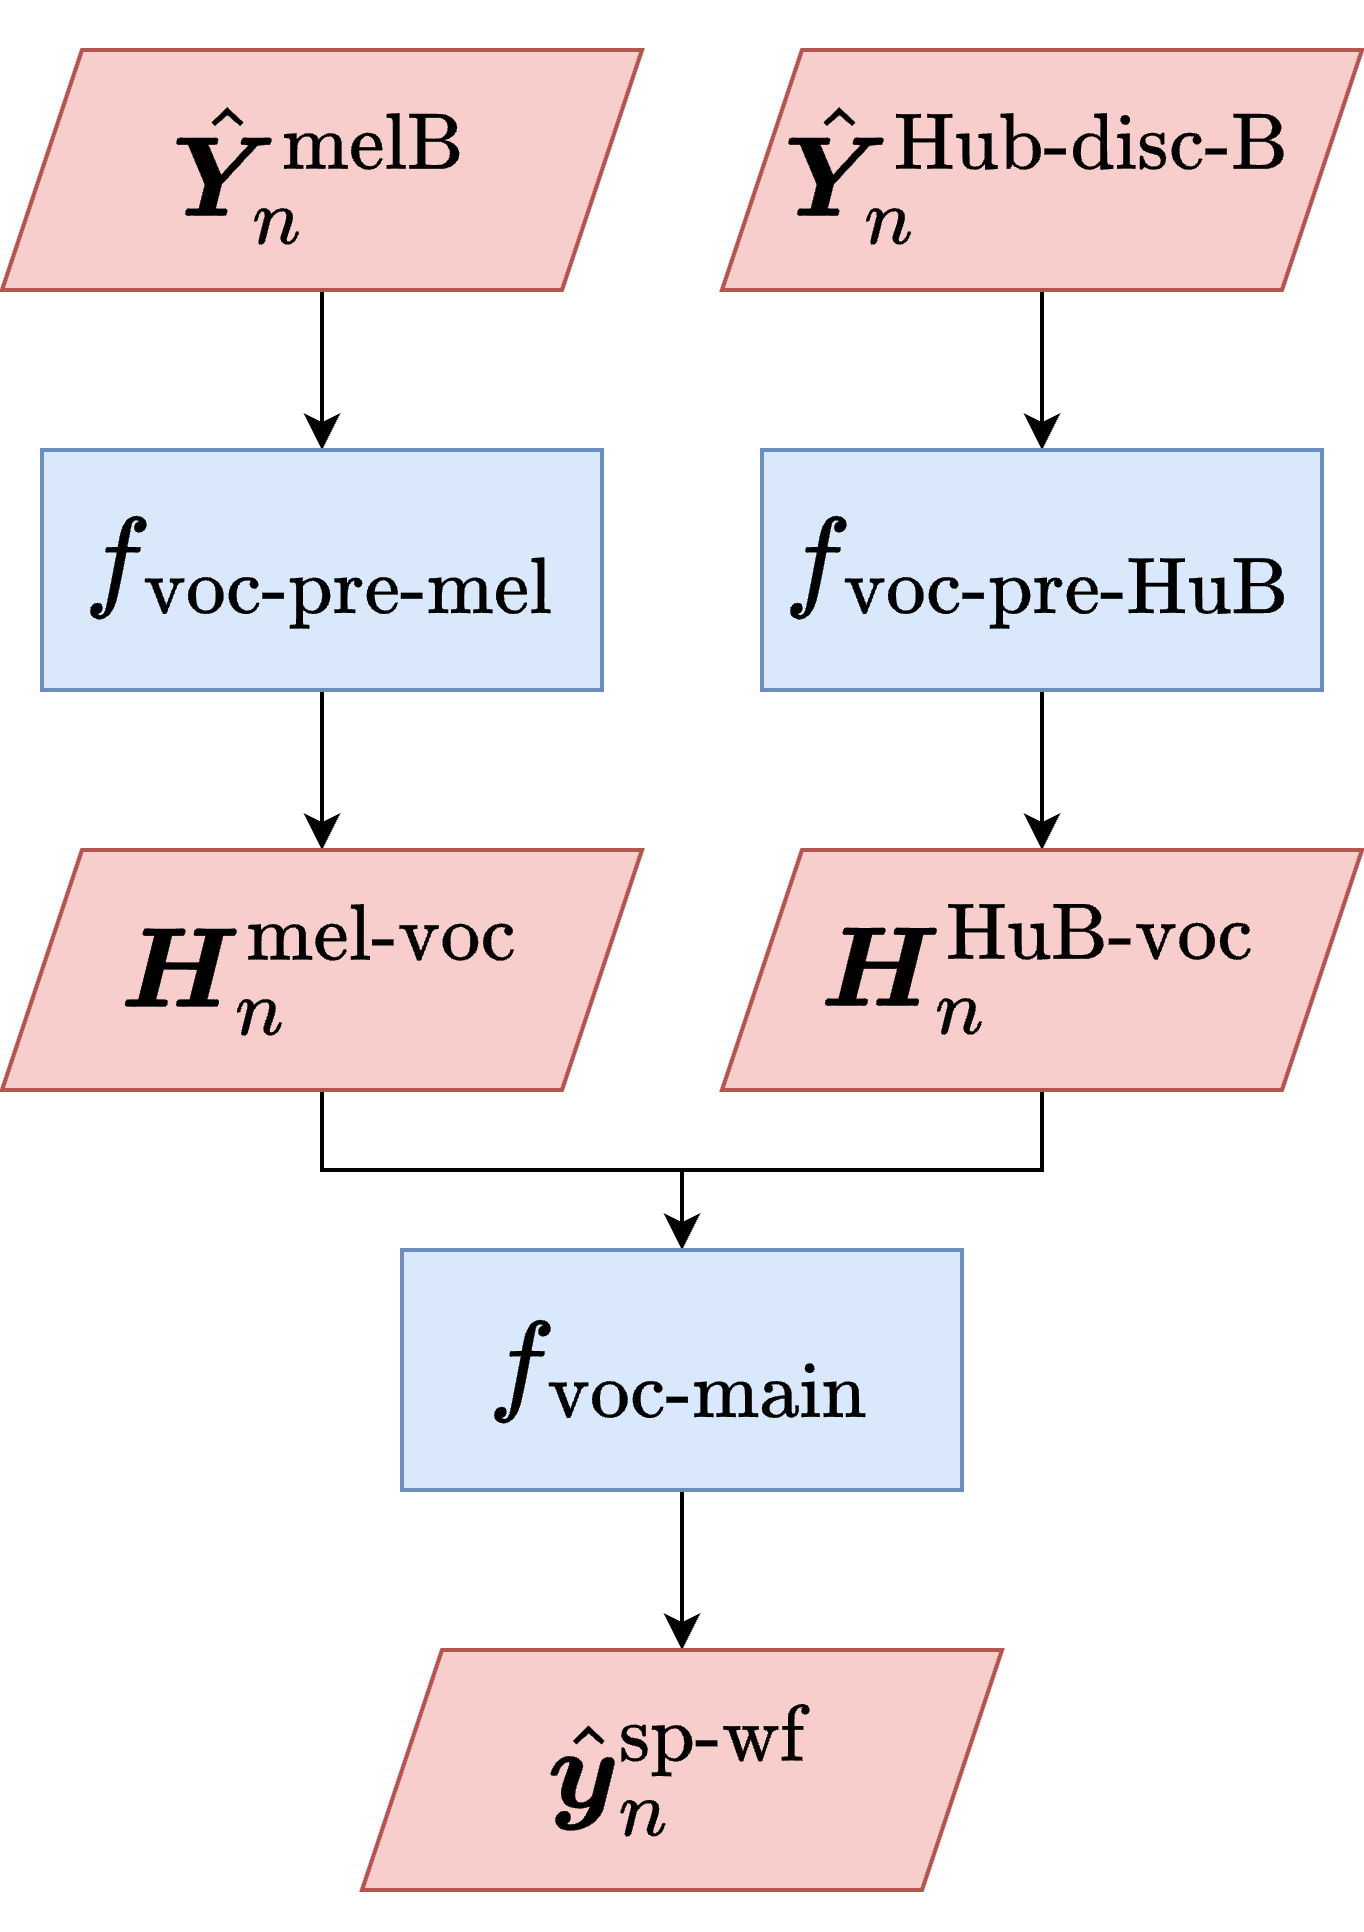
\includegraphics[width=45mm]{./figure/sec4/model_2/vocoder.drawio.png}
        \caption{全体}
        \label{sec4:fig:vocoder_overview}
    \end{subfigure}
    \hfill
    \begin{subfigure}[b]{0.32\textwidth}
        \centering
        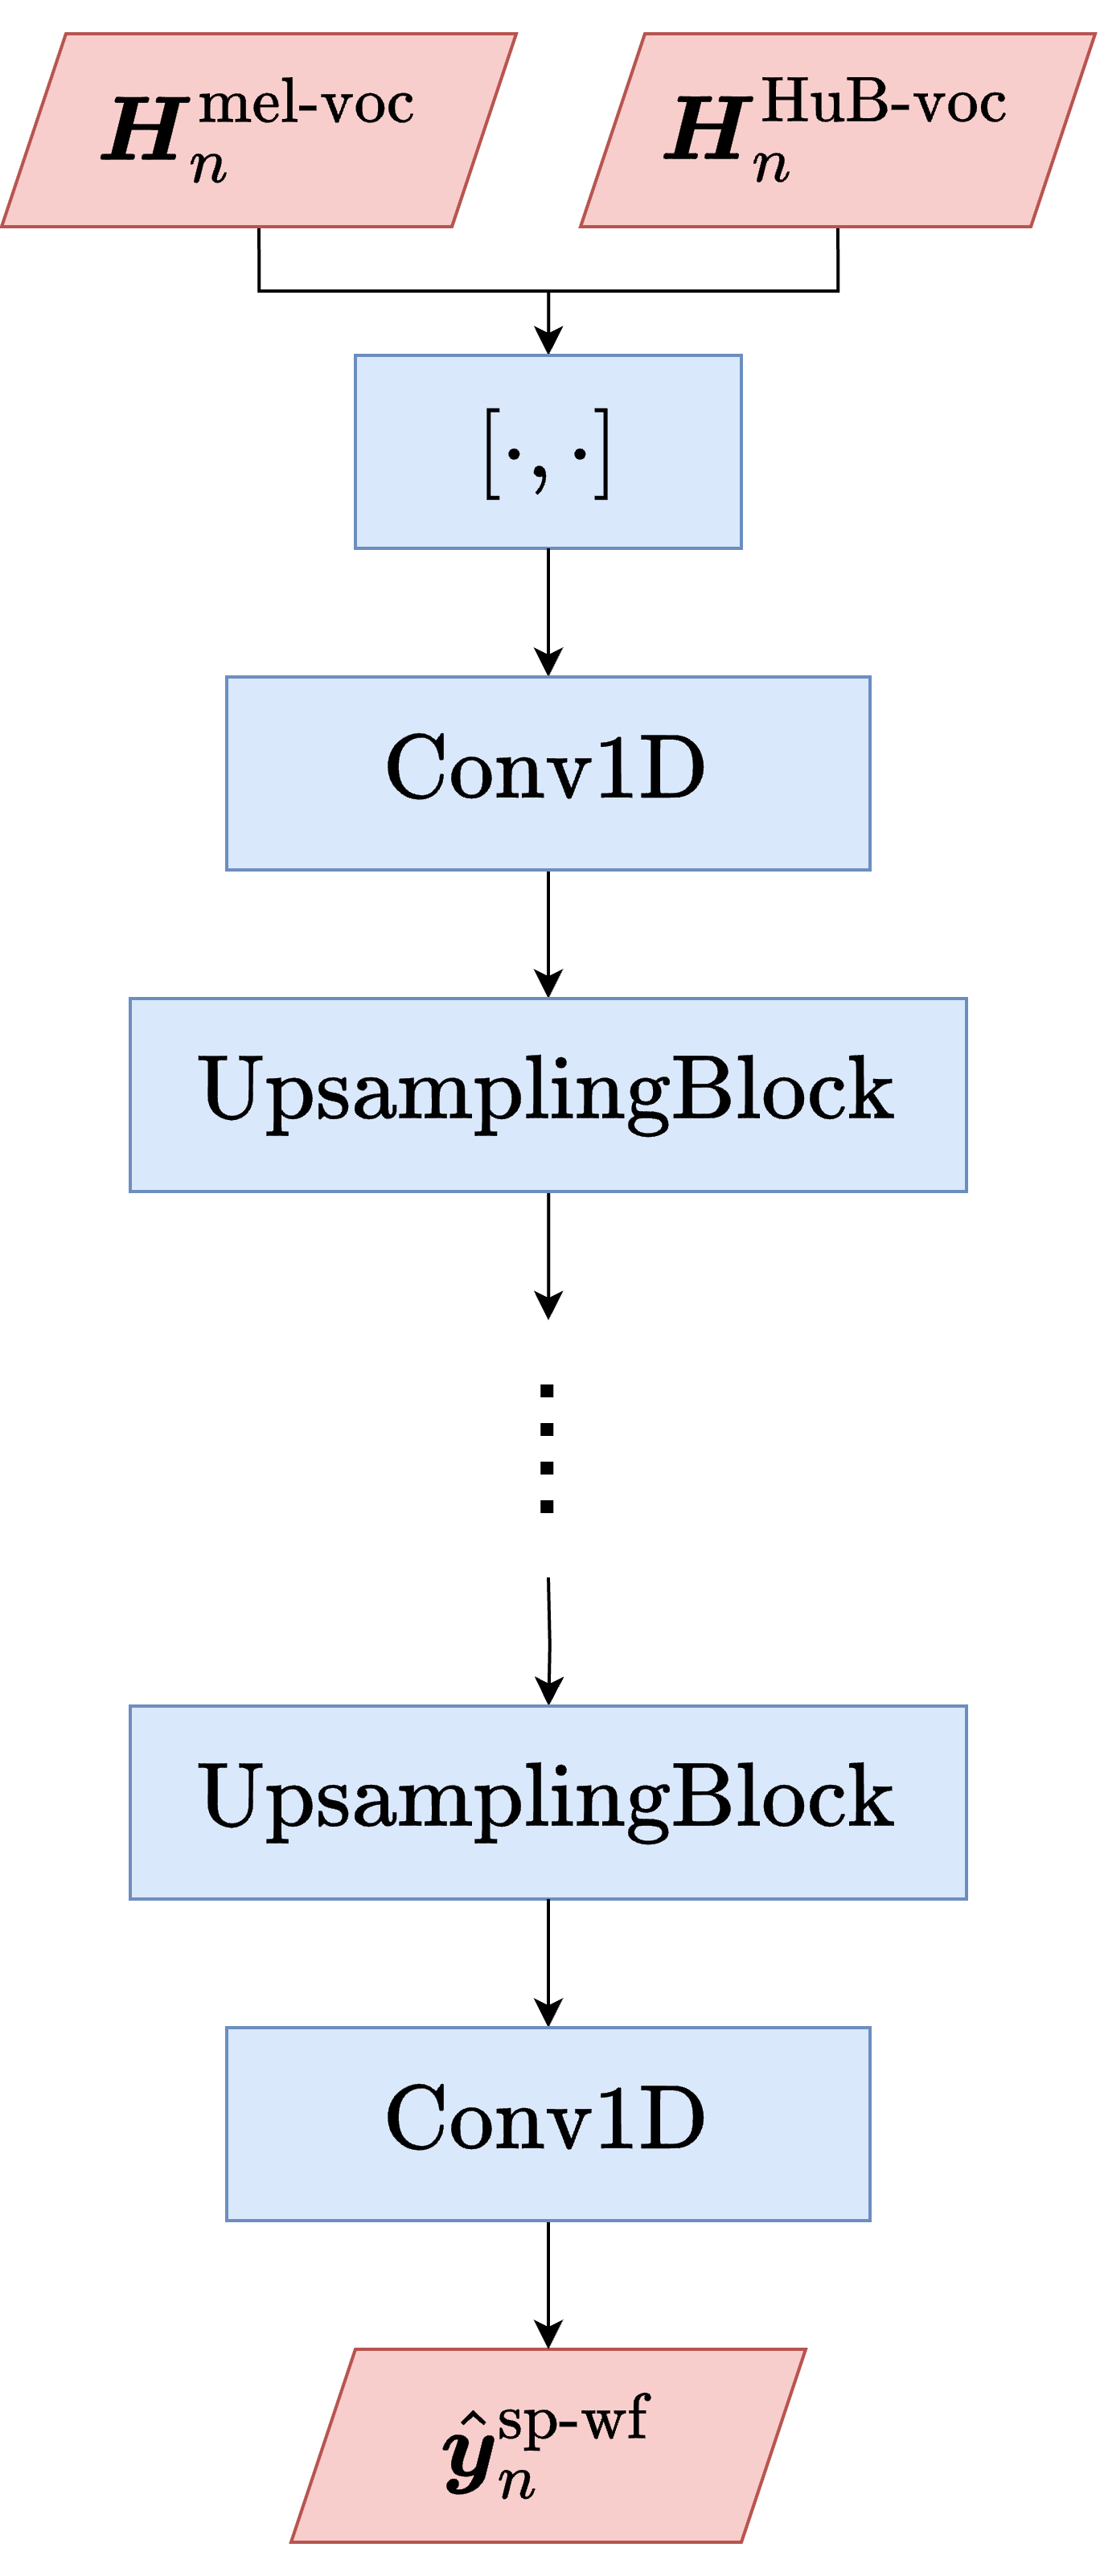
\includegraphics[width=45mm]{./figure/sec4/model_2/vocoder_main.drawio.png}
        \caption{$\vocoderMain$}
        \label{sec4:fig:vocoder_main}
    \end{subfigure}
    \hfill
    \begin{subfigure}[b]{0.32\textwidth}
        \centering
        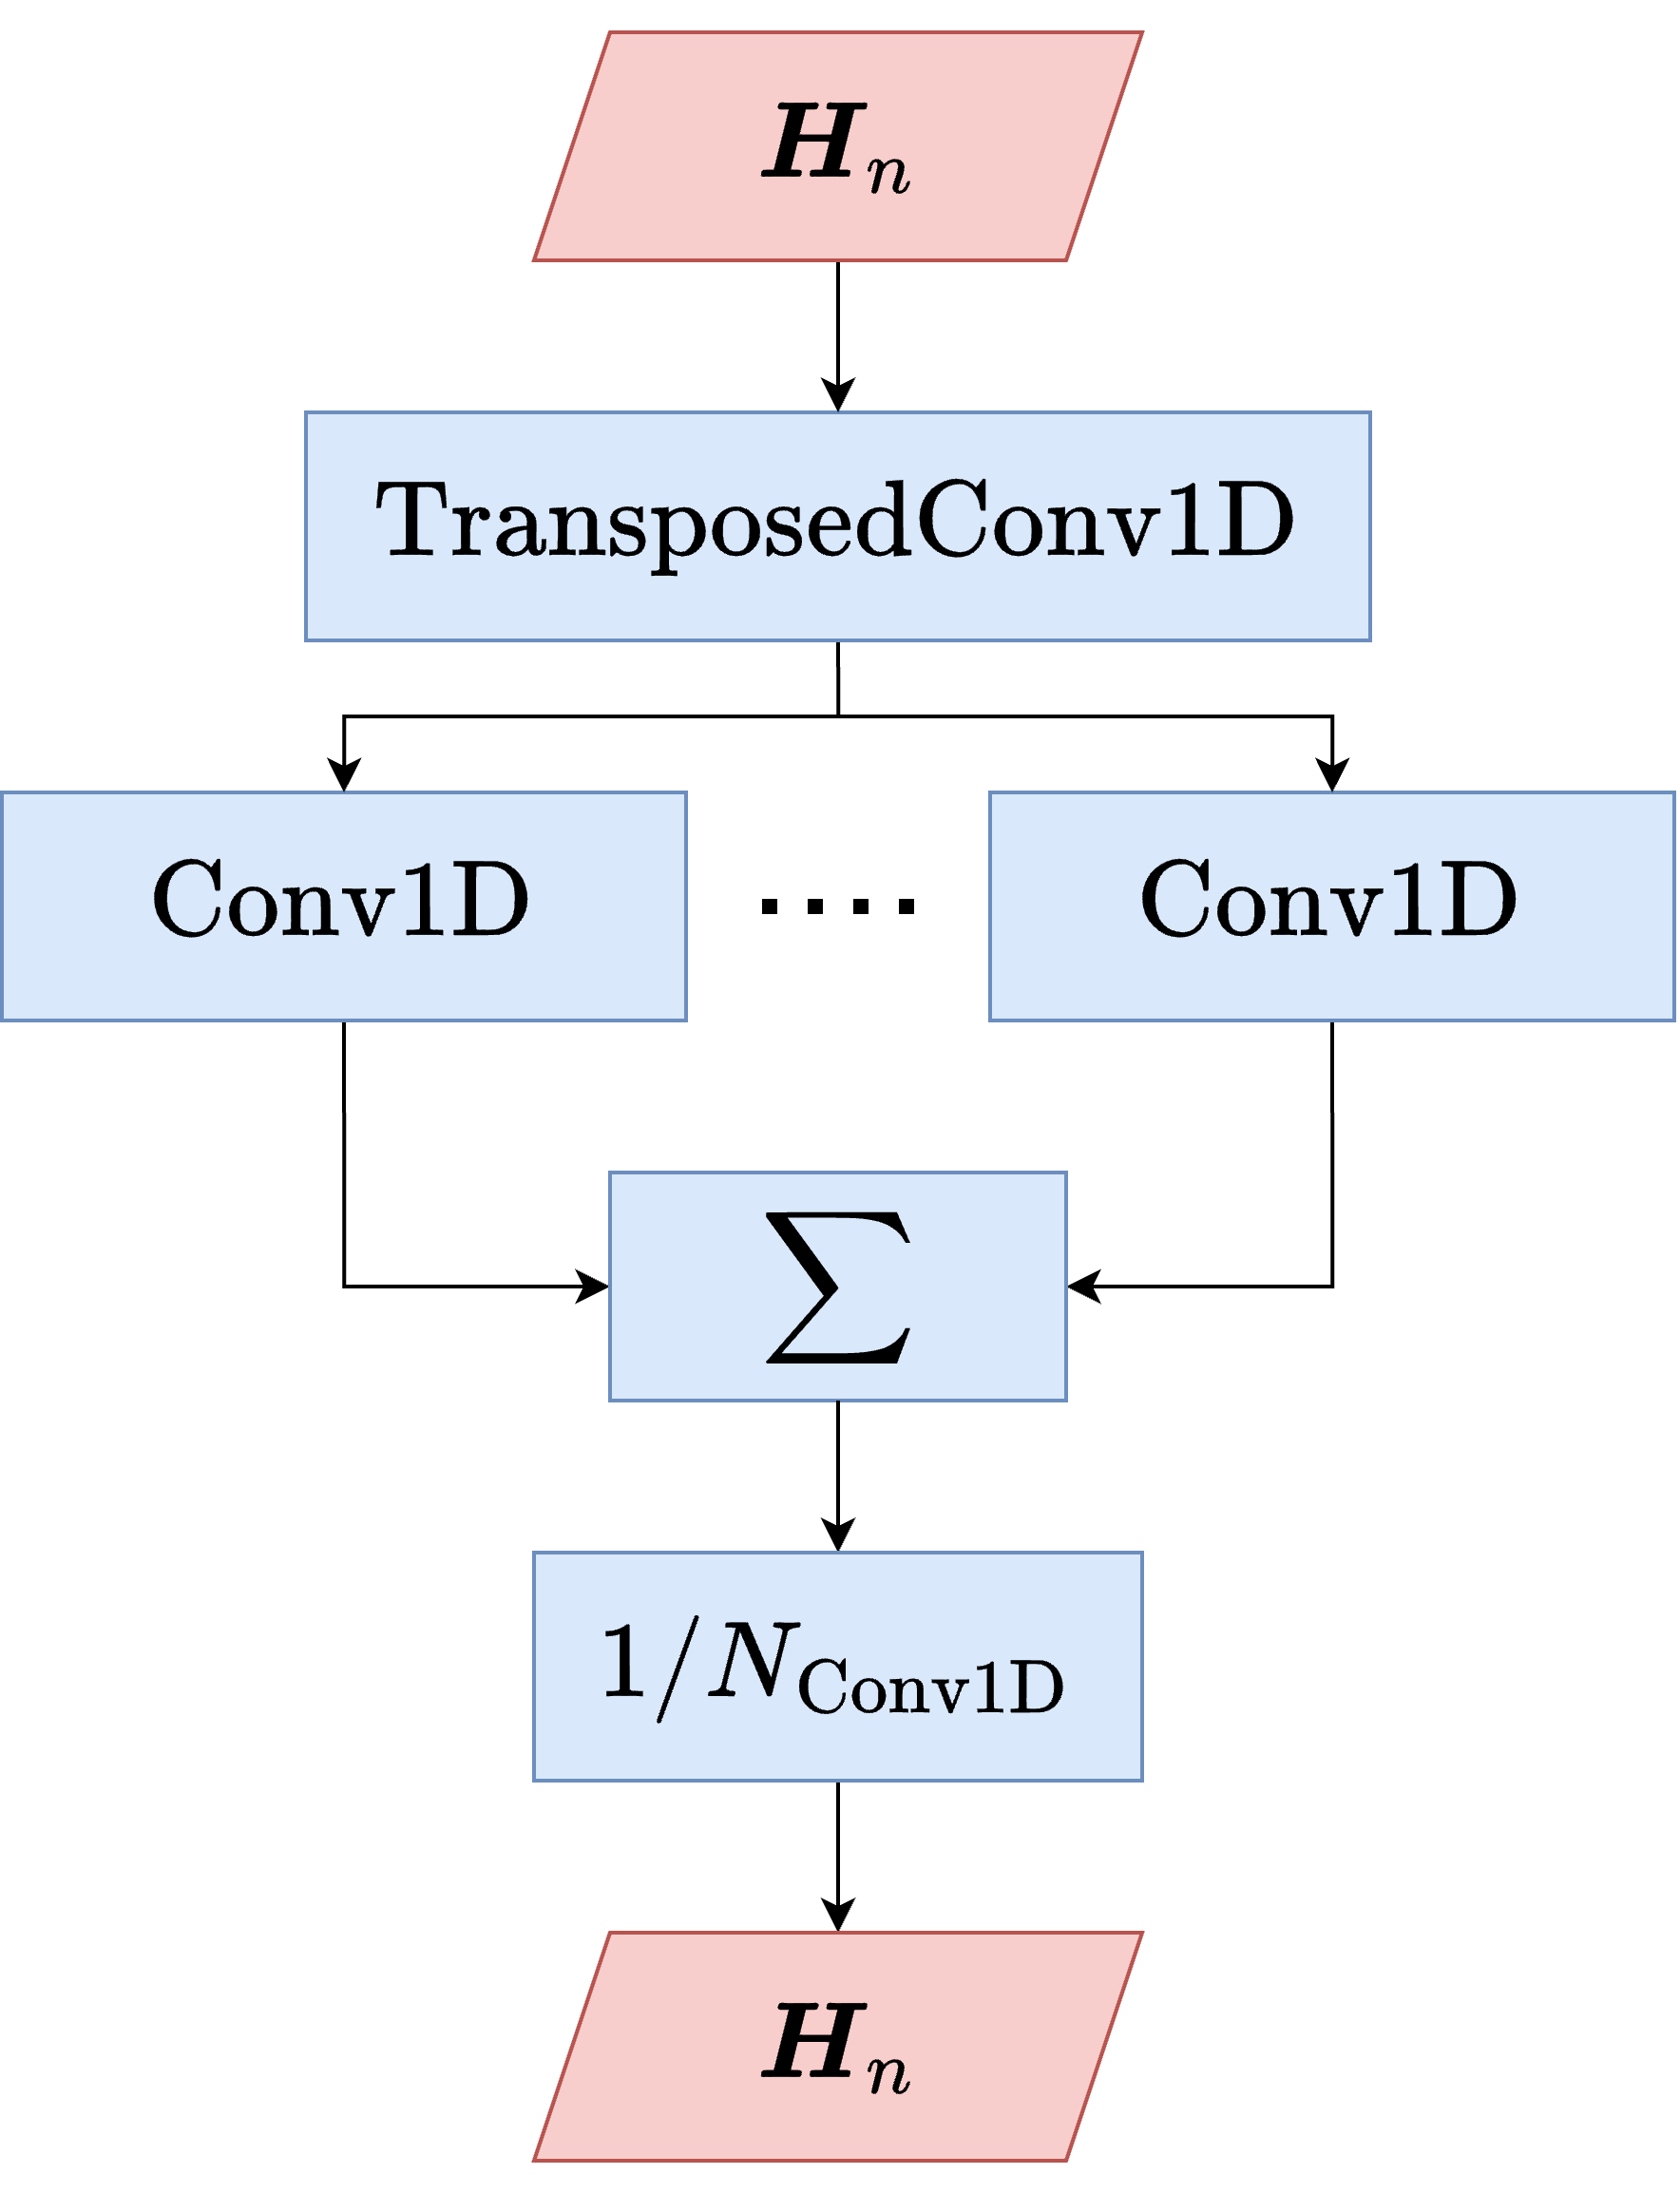
\includegraphics[width=45mm]{./figure/sec4/model_2/vocoder_main_block.drawio.png}
        \caption{UpsamplingBlock}
        \label{sec4:fig:vocoder_main_block}
    \end{subfigure}
    \caption{ボコーダの構造(赤い平行四辺形:入出力,青い長方形:処理)}
    \label{sec4:fig:vocoder}
\end{figure}

\subsubsection{損失関数}
まず,ネットワークAの学習に用いる損失関数$\lossA$は,
\begin{equation}
    \begin{aligned}
        \lossA & \lr{\hubertIntGt, \hubertIntPred, \melGt, \melPredA, \hubertDiscGt, \hubertDiscPredA}                 \\
        =      & \lossWeightHubInt \lossMAE{\hubertIntGt}{\hubertIntPred} + \lossWeightMel \lossMAE{\melGt}{\melPredA} \\
               & + \lossWeightHubDisc \lossCE{\hubertDiscGt}{\hubertDiscPredA}
    \end{aligned}
\end{equation}
で与えられる.すなわち,HuBERT中間特徴量についてのMAE Loss,メルスペクトログラムについてのMAE Loss,HuBERT離散特徴量についてのCross Entropy Lossの重み付け和である.

次に,ネットワークBの学習に用いる損失関数$\lossB$は,
\begin{equation}
    \begin{aligned}
        \lossB & \lr{\melGt, \melPredB, \hubertDiscGt, \hubertDiscPredB}                                                  \\
        =      & \lossWeightMel \lossMAE{\melGt}{\melPredB} + \lossWeightHubDisc \lossCE{\hubertDiscGt}{\hubertDiscPredB}
    \end{aligned}
\end{equation}
で与えられる.すなわち,メルスペクトログラムについてのMAE Loss,HuBERT離散特徴量についてのCross Entropy Lossの重み付け和である.

最後に,ボコーダの学習に用いる損失関数について,これはHiFi-GANと同様に,音声波形をメルスペクトログラムに変換して計算されるMAE Loss(元論文ではL1 Lossの期待値として定義される)と,Multi-scale Discriminator(MSD)およびMulti-period Discriminator(MPD)を用いて計算されるGAN Loss,Feature Matching Lossの重み付け和とした.